\documentclass[a4paper,11pt]{article}
\usepackage[utf8]{inputenc}
\usepackage[T1]{fontenc}
\usepackage{amsmath}
\usepackage{mathtools}
\usepackage{amsfonts}
\usepackage{amssymb}
\usepackage{graphicx}
\usepackage{multicol}
\usepackage{array}
\usepackage{float}
\usepackage{epstopdf}
\usepackage{caption}
\usepackage{subcaption}
\usepackage{gensymb}
\usepackage[bottom]{footmisc}
\usepackage{appendix}
\usepackage{pdfpages}
\usepackage{todonotes}
\usepackage{mathpazo}
\usepackage{titleps}
\usepackage{color}
\usepackage{xcolor}
\usepackage{colortbl}
\usepackage{siunitx}
\usepackage{pdflscape}
\usepackage{cancel}

\usepackage[skins]{tcolorbox}
\usepackage{sectsty}
\usepackage[arrowmos]{circuitikz}
\usepackage{pgfplots}
\usepackage{blindtext}
\usepackage[inner=2cm,outer=2cm,top=2.5cm,bottom=2.5cm]{geometry}
\usepackage{todonotes}
\usepackage{hyperref}
\usepackage{url}
\usepackage{adjustbox}
\usepackage{tabularx}
\usepackage{booktabs}
\usepackage{fancybox}
\usepackage[tikz]{bclogo}



%For code insertion
%listing
\usepackage{listings}
\usepackage{xcolor}
\definecolor{codegreen}{rgb}{0,0.6,0}
\definecolor{codegray}{rgb}{0.5,0.5,0.5}
\definecolor{codepurple}{rgb}{0.58,0,0.82}
\definecolor{backcolour}{rgb}{0.98,0.98,0.98}
\lstdefinestyle{mystyle}{
    backgroundcolor=\color{backcolour},
    commentstyle=\color{codegreen},
    keywordstyle=\color{blue},
    numberstyle=\tiny\color{codegray},
    stringstyle=\color{codepurple},
    basicstyle=\ttfamily\footnotesize,
    breakatwhitespace=false,
    breaklines=true,
    captionpos=b,
    keepspaces=true,
    numbers=left,
    numbersep=5pt,
    showspaces=false,
    showstringspaces=false,
    showtabs=false,
    tabsize=2
}
\lstset{style=mystyle}



\graphicspath{{figures/}}
\sectionfont{\large}
\subsectionfont{\normalsize}


\newpagestyle{main}{
	\sethead[LELEC2103][][]{LELEC2103}{}{}
	\headrule
    \setfoot[][\thepage][]{}{\thepage}{}
}

\newcommand{\horrule}[1]{\rule{\linewidth}{#1}} % Create horizontal rule command with 1 argument of height

%%%%%%%%%%%%%%%%%%%%%%%%%%%%%%%%%%%%%%%%%%%%%%%%%%%%%%%%%%%%%%%%%%%%%%%%%%%%

\begin{document}
\renewcommand{\figurename}{Fig.}

\renewcommand{\thepage}{\arabic{page}}
\setcounter{page}{1}
\pagestyle{main}
\newpage \clearpage

\begin{center}
\begin{LARGE}
LELEC2103: Optimization
\end{LARGE}
\vspace{0.3cm}
%\textit{TA 1, TA 2}
\end{center}

\section{Signal processing}
The space for improvement in the signal processing parts is very large.
Actually, you can consider any possible function that maps an audio sequence to an integer giving the predicted class. The only contextual constraint is that you must send somehow the acquired information wirelessly from the transmitter to the receiver. Then you also have to take into account the physical constraints imposed by your devices in terms of sampling, processing, memory, data rate and energy consumption. The priority when optimizing a working project is to identify the bottlenecks, i.e. the parts that are the most limiting the performances. Think about it before spending 3 weeks on something which would give negligible improvements at the end. To organize your reasoning, you can decompose the signal processing (without the authentication and packet creation aspects) in three main steps:

%%%%%%%%%%%%%%%%%%%%%%%%%%%%%%%%%%%%%%%%
\subsection{Feature vector shaping}
%%%%%%%%%%%%%%%%%%%%%%%%%%%%%%%%%%%%%%%%

\begin{figure}[H]
    \centering
    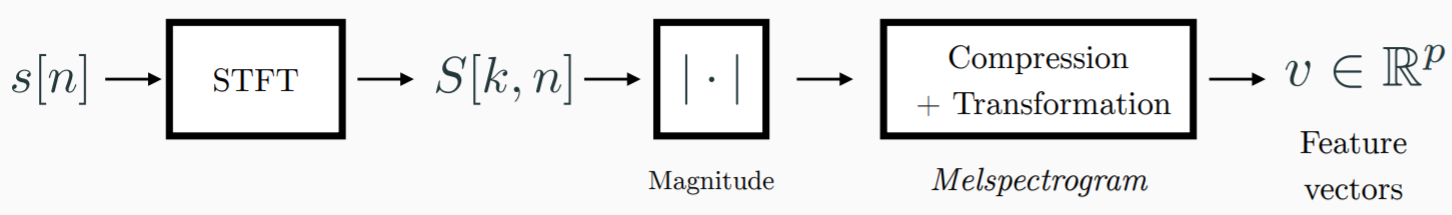
\includegraphics[width=14cm]{figs/scheme.PNG}
    \caption{Computation chain from temporal audio signal to feature vector.}
    \label{fig: fv}
\end{figure}
During the first semester, we provided you with a time-frequency representation that was compressed using the Hz$\rightarrow$mel transformation, as depicted in Figure \ref{fig: fv}. This choice is interesting because it yields intuitive observations and results for a human. To optimize this step, you can consider another block scheme. You could for instance choose another way of compressing the information than using Mels. Or you could keep a pure temporal representation and compress it another way.
However, this is not compulsory and we argue the current scheme in Figure \ref{fig: fv} is already efficient. \\
What can be done is to keep this scheme and play with its parameters. You can vary the window size and shape for the STFT. You can vary the number of mels. And mainly, these computations are all made in C code in a fixed-point representation. We voluntarily wrote non optimal code. \\
Finally, a way to save energy on your device is to avoid computing feature vectors when you think the currently acquired sound does not contain anything important. A first approach we can think of is an energy threshold, where we decide not to compute the feature vector if the sound is not loud enough.

To synthesize, some options are:
\begin{itemize}
    \item Change the feature vector computation scheme.
    \item Optimize this scheme by tuning its parameters and improving the
    fixed-point implementation.
    \item Imagine criteria for starting the computation of the feature vector.
\end{itemize}
%
%%%%%%%%%%%%%%%%%%%%%%%%%%%%%%%%%%%%%%%%
\subsection{Classification}
%%%%%%%%%%%%%%%%%%%%%%%%%%%%%%%%%%%%%%%%

\begin{figure}[H]
    \centering
    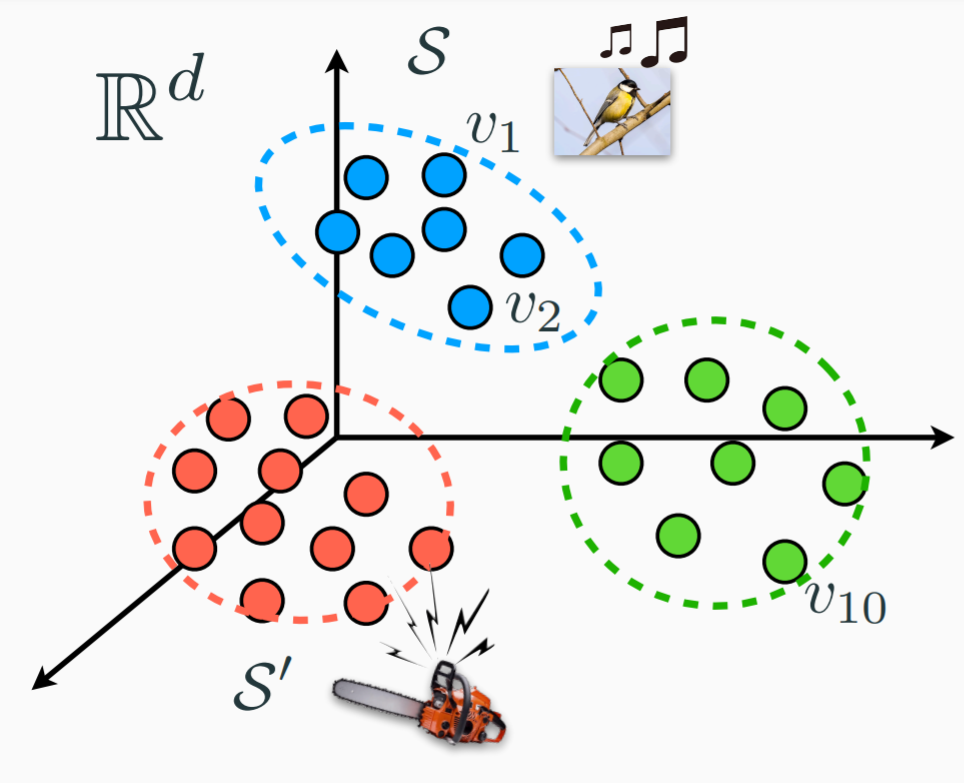
\includegraphics[width=8cm]{figs/classification.PNG}
    \caption{Classification principle.}
    \label{fig: classification}
\end{figure}
Once the feature vector computation process is fixed, the information contained in this feature vector has to be exploited at the receiver side for the classification, as shown in Figure \ref{fig: classification}. During the first semester, we already let you the possibility to play with different simple classifiers. The choice of the classifier is crucial and we advise you to test even more sophisticated ones to boost your perfomances. But remember to avoid overfitting! \\
You could consider the possibility to have a confidence metric on your predictions (remember that most classifiers provide first a probability of correct classification before to make a decision). This can be accompanied by a way to strenghten this confidence with the increasing amount of information provided by new features vectors. \\
Until now, you are classifying no matter what. There are situations where it is preferable not to output a prediction (i) the energy of the acquired sound is too low and you don't want to compute the feature vector on it (ii) your classifier outputs a probability vector balanced and no class is really highlighted. You are encouraged to manage these situations for the end of this project.


To synthesize, some options are:
\begin{itemize}
    \item Change the classifier.
    \item Add a confidence metric and exploit time to increase this confidence.
    \item Consider a threshold to output no class.
\end{itemize}

%%%%%%%%%%%%%%%%%%%%%%%%%%%%%%%%%%%%%%%%
\subsection{Training data}
%%%%%%%%%%%%%%%%%%%%%%%%%%%%%%%%%%%%%%%%

The way you train your classification model in this project is by using labelled (or training) data. This data is as important as the classifier choice. During the first semester, you trained your model with clean audio samples from the ESC-50 dataset, and discovered the possibility to augment this data by adding some transformations aiming to mimick real life perturbations. Now you master your devices and acquisition procedures, a better option is to create training data using your device. It implicitely takes the acquisition non idealities into account, and gives you the possibility to truly augment the data increasining the distance between the sound source and microphone, or adding background sound by yourself. \\
\\
Don't hesitate to discuss all your ideas with the TA's!

\newpage
\section{Crypto - Security analysis}
Let us assume that our system is deployed with multiple sensor nodes that all
share the same key.
We ask you to analyze the \textbf{security} properties of the system against the
following attacks:
\begin{itemize}
    \item Forgery of packets using a wrong key.
    \item CBC-MAC length extension attack.
    \item CBC-MAC padding attack.
    \item Transmitter modification attack (capture a packet sent by the device
        while jamming the receiver, and re-emit the packet, while changing the
        \texttt{emitter\_id}).
    \item Packet replay attack (capture a packet sent by a device, and re-emit
        it later).
    \item Packet delay attack (capture a packet sent by the device while
        jamming the receiver, and re-emit the packet later).
    \item Eavesdropping attack: capture the packets and extract information.
    \item Timing attack against the AES implementation.\footnote{%
            For more information of timing attacks, see~\url{%
                https://en.wikipedia.org/wiki/Timing_attack
            } and, for more details,
            \url{http://citeseerx.ist.psu.edu/viewdoc/download?doi=10.1.1.42.679&rep=rep1&type=pdf}
            (the AES block cipher was originally named Rijndael).
        }
\end{itemize}

\noindent For each of those attacks, describe
\begin{itemize}
    \item the plausible goals of an adversary that would mount such an attack
        (perform this analysis while considering that the system monitors a
        forest),
    \item whether the attack is possible to mount, and what capabilities would the
        adversary need to mount the attack (Justify your claim based on your
        understanding of the system and support your claims by analysis of the
        code (running on the MCU or on the receiver) or by experimental
        evidence.),
    \item if the attack is possible to mount, analyze whether protecting
        against it would require a packet format change (with respect to the format
        given in H6,
        or if the packet can be kept unchanged, and only the emitter or
        receiver implementation have to be changed.
\end{itemize}
\noindent The report concerns security at the cryptographic level. Thus, assume for all cases the following :
\begin{itemize}
\item The adversary knows every detail of the implementation, packet format and so on. Only the secret shared key is hidden from the adversary.
\item The receiver node is able to process all incoming packets, therefore jamming and denial of service are out of scope.
\end{itemize}
Finally, be brief and limit yourselves to the one attack listed above at a time (i.e. don't use them as basis for other attacks.). Every attack can be analyzed and justified in a couple of lines.

\begin{bclogo}[couleur = gray!20, arrondi = 0.2, logo=\bcinfo]{AES timing attack vulnerability}
    If the execution time of the implementation of a cryptographic primitive
    depends on the key, then it is vulnerable to timing attacks.
    In order to test this property for the AES implementation you use, you need
    perfectly repeatable (i.e., noise-free) measurements of the execution time
    of the AES encryption function. (The \texttt{\_\_disable\_irq();} and
    \texttt{\_\_enable\_irq();} macros may be useful.)
    Then measure the execution time for various keys and quantify its variability.
\end{bclogo}


\end{document}
%%%%%%%%%%%%%%%%%%%%%%%%%%%%%%%%%%%%%%%%%%%%%%%%%%%%%%%%%%%%%%%%%%%%%%%%%%%%
